%%%%%%%%%%%%%%%%%%%%%%%%%%%%%%%%%%%%%%%%%
% Facial Expresion Recognition with Convolutional Neural Networks
% 
% Lewe Ohlsen
% Fachhochschule Wedel
%
% Latex Template by Frits Wenneker (http://www.howtotex.com)
%
%%%%%%%%%%%%%%%%%%%%%%%%%%%%%%%%%%%%%%%%%

%----------------------------------------------------------------------------------------
%	PACKAGES AND OTHER DOCUMENT CONFIGURATIONS
%----------------------------------------------------------------------------------------

\documentclass[twoside]{article}

\usepackage{lipsum} % Package to generate dummy text throughout this template
\usepackage{graphicx} % Figures from matplotlib
\graphicspath{ {figures/} }

\usepackage[sc]{mathpazo} % Use the Palatino font
\usepackage[T1]{fontenc} % Use 8-bit encoding that has 256 glyphs
\linespread{1.05} % Line spacing - Palatino needs more space between lines
\usepackage{microtype} % Slightly tweak font spacing for aesthetics

\usepackage[hmarginratio=1:1,top=32mm,columnsep=20pt]{geometry} % Document margins
\usepackage{multicol} % Used for the two-column layout of the document
\usepackage[hang, small,labelfont=bf,up,textfont=it,up]{caption} % Custom captions under/above floats in tables or figures

\usepackage{booktabs} % Horizontal rules in tables
\usepackage{float} % Required for tables and figures in the multi-column environment - they need to be placed in specific locations with the [H] (e.g. \begin{table}[H])
\usepackage{hyperref} % For hyperlinks in the PDF
\usepackage{cite} % BibTex

\usepackage{paralist} % Used for the compactitem environment which makes bullet points with less space between them

\usepackage{abstract} % Allows abstract customization
\renewcommand{\abstractnamefont}{\normalfont\bfseries} % Set the "Abstract" text to bold
\renewcommand{\abstracttextfont}{\normalfont\small\itshape} % Set the abstract itself to small italic text

\usepackage{titlesec} % Allows customization of titles
\usepackage[utf8]{inputenc}
%\renewcommand\thesection{\Roman{section}} % Roman numerals for the sections
%\renewcommand\thesubsection{\Roman{subsection}} % Roman numerals for subsections
\titleformat{\section}[block]{\large\scshape\centering\bfseries}{\thesection.}{1em}{} % Change the look of the section titles
\titleformat{\subsection}[block]{}{\thesubsection.}{1em}{} % Change the look of the section titles


%----------------------------------------------------------------------------------------
%	TITLE SECTION
%----------------------------------------------------------------------------------------

\title{\vspace{-15mm}\fontsize{16pt}{10pt}\selectfont\textbf{Facial Expression Recognition with\\ Convolutional Neural Networks}} % Article title 

\author{
	\large
	\textsc{Lewe Ohlsen}\\[2mm] % Your name
	\normalsize Fachhochschule Wedel \\ % Your institution
	\normalsize \href{mailto:minf101062@fh-wedel.de}{minf101062@fh-wedel.de} % Your email address
	\vspace{-5mm}
}
\date{}

%----------------------------------------------------------------------------------------

\begin{document}

\maketitle % Insert title

%----------------------------------------------------------------------------------------
%	ARTICLE CONTENTS
%----------------------------------------------------------------------------------------

\begin{multicols}{2} % Two-column layout throughout the main article text

\section{Introduction}

Automatically recognizing facial expressions is an interesting and challenging problem in the field of human computer interaction. Facial expressions can be interpreted and categorized into six classes of basic emotion that seem to be found across all human cultures: anger, disgust, fear, happiness, sadness, and surprise \cite{ekman93}. This projects goal is to develop a classifier for real-time detection of these facial expressions using deep learning.

%------------------------------------------------

\section{Related work}
In the last years, great progress was made on the problem of automatically detecting facial expression from images. Some researchers have attempted to derive emotions from detecting individual muscle movements in images of faces by identifying muscles and their degree of activation \cite{lien98}. However, manually extracting the muscle activations from a set of images requires expert knowledge or complex algorithms. With Convolutional Neural Networks (CNNs), training data only consists of images along with matching class labels that describe the images. Relevant features, such as a smile that implies happiness, are learned implicitly and do not require manual extraction. CNNs have been used successfully for various image recognition tasks, including facial expression recognition \cite{dumas01}. The aim of this work was to test how well multiple CNN models, trained on different datasets, perform together on the task of recognizing facial expressions.
%------------------------------------------------

\section{Datasets}
To train an automatic classifier using deep learning technology, a dataset with samples that describe the problem is required. Each image in the dataset is mapped to an integer class label 0–6 for the corresponding emotion. Two datasets, FER2013 \cite{goodfel13} and CK+ \cite{cohn00} are considered for training the deep learning model.

\begin{figure}[H]
	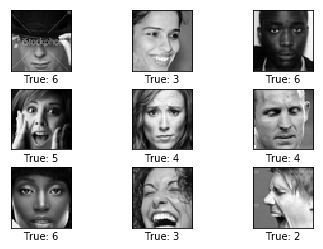
\includegraphics[width=0.48\textwidth]{fer_examples}
	\caption{FER-2013 training samples}
\end{figure}


\subsection{FER-2013}
The FER-2013 dataset consists of roughly 37.000 images showing faces of people expressing a certain emotion. Most of the 48x48 pixel grayscale images are stock footage. All images have been centered on the persons faces to show a similar region in every sample. As this has been done automatically, some images are not centered correctly. Persons are depicted from different camera angles, some faces are occluded and rotation is different across the images. These circumstances make the problem of generalizing on the training data difficult. 

The class labels were crowd-sourced with Amazon Mechanical Turk, where quality work is not incentivized, so faulty labels are likely a problem. It is expected that every subject shows only a single emotion, where in reality faces can express at least two emtions simultaniously (e.g happiness and surprise). To resolve this problem and improve the overall quality of the FER-2013 dataset, a research group at Microsoft worked on re-labeling the dataset \cite{barsoum16}: To get a better approximation of the ground-truth emotions, ten workers on Mechanical Turk were asked to label each image. Instead of single class labels, probability distributions of emotion classes describe each persons facial expression.

\begin{figure}[H]
	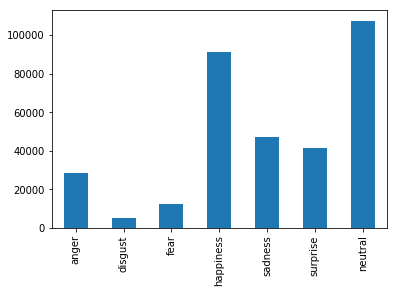
\includegraphics[width=0.48\textwidth]{ferplus_distribution}
	\caption{FER-2013 dataset class distribution}
\end{figure}

\subsection{Cohn-Kanade (CK+)}
To augment the wild variety of FER-2013 images, a second, more conservative dataset with only frontal faces is used to train a second classifier. The Cohn-Kanade (CK+) dataset consists of 593 image sequences across 123 subjects. Each image sequence goes from a neutral facial expression to a posed "peak expression" according to the six basic emotions. Only 327 of the 593 image sequences are labeled with emotion data. This is because not all images fit the prototypic definition of the Facial Action Coding System (FACS). CK+ also comes with FACS data, where facial action units (e.g raised eyebrow) are identified along with their degree of activation.

\begin{figure}[H]
	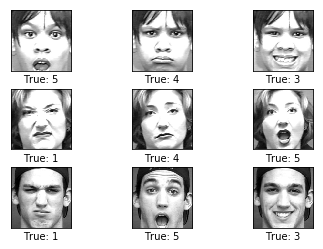
\includegraphics[width=0.48\textwidth]{ckplus_examples}
	\caption{Posed facial expressions from the CK+ dataset}
\end{figure}

%------------------------------------------------

\section{Convolutional Neural Networks (CNNs)}
Convolutional Neural Networks are a special kind of multi-layer artificial neural networks. CNNs have been around since the 1990s \cite{lecun98}, however they have lead to breakthrough results in practical application with computational power becoming more affordable in the last years. Convolutional Neural Networks can recognize visual patterns directly from pixel images with very little preprocessing. 

Like a regular Artificial Neural Network, a CNN can be thought of as a function $f(x) = y$ where the input $x$ is an image of a face and $y$ is a probability distribution of the classes this image is predicted to belong to (e.g happiness, surprise, sadness). Input images are flattened in dimension from 48x48 pixels to a single 2304-dimensional vector. For training and predictions, multiple images can be fed into the neural network at once.

The model function is implemented as a multi-layer computational graph where transformations are applied to the input on every layer.


\subsection{CNN Components}

\subsubsection{Convolutional Layer}
The convolutional layer is the core building block of a CNN. Each layer is initialized with a set of $n$ random two-dimensional filter matrices (eg 3x3 pixels) and a pixel-stride. When an image is put into the convolutional layer, each of the filters is moved across the height and width of the image, calculating a dot product between the filter matrix and the current section of the image. The resulting matrices of dot products are called feature maps. \cite{karpathy} To introduce non-linearity to the model function, a ReLu activation function $f(x) = max(0, x)$ is used on the feature-maps element-wise. The filters in the convolutional layers are trained using the backpropagation algorithm \cite{goodfel16}. Intuitively, filters activate when they see different types of visual features, such as vertical or diagonal edges on the lower layers or more complex patterns like eyes or mouths in the top convolutional layers.

\subsubsection{Pooling Layer}
To down-sample images between the layers in favor of making the training process faster, pooling layers are introduced in the computational graph. Similar to the convolutional layer, filters are moved across the layer input, executing a pooling operation on each position. A common pooling operation is taking the max value on every filter position (Max-Pooling). For instance when pooling with a filter size of 2x2 pixels and a stride of 2 is applied to a 48x48 pixels image, the pooling output is a 24x24 pixels image.

\subsubsection{Fully-Connected layers}
In CNNs, fully connected layers are added at the top of the network. The advanced features that have been extracted in the top convolutional layers are usually connected to two or more layers of weighted nodes. On the first fully-connected layer, linear combinations of the feature maps activations are created. Intuitively, combinations of filters are mapped to emotion class probabilities. A softmax function can be applied on the output layer to normalize the topmost fully connected layer into a valid probability distribution.


%------------------------------------------------

\section{Model Architecture and Training}
To effectively reduce dimensions between the input and output space and find a valid representation of the input image, a CNN is implemented using the TensorFlow higher-level APIs. The TensorFlow extimator API is used, which provides a convenient abstraction layer by encapsulating trainable classifiers.

In simple CNNs, it is common to combine convolutional and pooling layers to compute feature activations while reducing dimensionality. During the designing process, it turned out that stacking multiple convolutional layers improved the model accuracy on the test set by about 20 percent compared to alternating pooling and convolutional layers. This is because the pooling operation causes loss of information and multiple adjacent convolutional layers allow more complex filters to emerge.

The model architecture has been improved incrementally throughout the designing process. Hyperparameter optimization has not been done programmatically but rather by trial-and-error.

\bigskip

\begin{tabular}{|| c ||}

  \hline
  FC [7 nodes] output\\
  FC [1024 nodes]\\
  \hline
  MAX POOL [2x2 pixels, stride 2]\\
  CONV [256 filters, 3x3 pixels]\\
  CONV [256 filters, 3x3 pixels]\\
  CONV [256 filters, 3x3 pixels]\\
  \hline
  MAX POOL [2x2 pixels, stride 2]\\
  CONV [128 filters, 3x3 pixels]\\
  CONV [128 filters, 3x3 pixels]\\
  CONV [128 filters, 3x3 pixels]\\
  \hline
  MAX POOL [2x2 pixels, stride 2]\\
  CONV [64 filters, 3x3 pixels]\\
  CONV [64 filters, 3x3 pixels]\\
  \hline
  MAX POOL [2x2 pixels, stride 2]\\
  CONV [32 filters, 3x3 pixels]\\
  CONV [32 filters, 3x3 pixels]\\
  \hline
    
\end{tabular}

\medskip

\textit{The final network architecture. Bottom-up from input to output.}


\subsection{Training Procedure}
The CNN is trained on a subset of 28221 training examples from the FER-dataset according to the original train-test-validation split. The FERplus prabability distributions are used as as labels. In the training subset, only images with a maximum label class probability of $> 0.5$ were considered. The CNN models filters and weights/biases of the fully connected layers are fit to the training set using the backpropagation algorithm. Therefore, a cross-entropy loss function is used to measure the model error and the Adam optimization algorithm with an initial step size of 0.001 is used to minimize the loss. To prevent overfitting the model on the training set, the loss value on the validation set (3532 unseen images) is computed periodically during training. When the validation loss stops decreasing, training is stopped and the final model accuracy is computed on a test subset.


%------------------------------------------------


\section{Results}
The final CNN model scored an accuracy of 73.2\% on a test-set of 3482 face examples. Training was executed on a shared Tesla K80 GPU instance by Google Colab \cite{colab}, a cloud powered, interactive Jupyter notebook environment. Training with 24 iterations over the training set (epochs) took about 15 minutes.

\begin{figure}[H]
	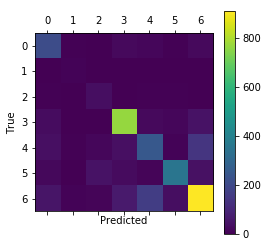
\includegraphics[width=0.48\textwidth]{confusion}
	\caption{Confusion matrix showing the accuracy for each class}
\end{figure}

Occlusion bla bla

\begin{figure}[H]
	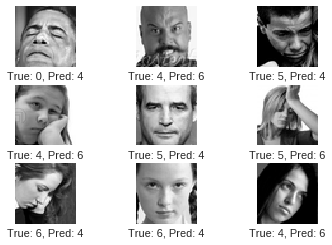
\includegraphics[width=0.48\textwidth]{errors}
	\caption{Examples of wrongly classified images}
\end{figure}


%------------------------------------------------

\section{Conclusion and Discussion}

% - CNN robustness to occlusion, distortions and geometric transformations.
In live predictions with a webcam, the classifier has shown to be accurate in most of the predictions. However, predictions for the classes $disgust$ and $fear$ are hard to reproduce. This is most likely because the seven classes of emotion in the dataset are highly imbalanced. For instance $disgust$ only has about 500 training samples while $happy$ has about 7000. This results in biased predictions with higher probabilities of the majority classes. In order to balance the training dataset, data augmentation \cite{krizhevsky12} could be used: To increase the number of training examples for a given class, the images could be flipped horizontally or rotated in multiple random angles. Given more time for this project, I would like to have experimented with such techniques of data augmentation and also with more complex model architectures.



%----------------------------------------------------------------------------------------
%	REFERENCE LIST
%----------------------------------------------------------------------------------------

\bibliography{paper}
\bibliographystyle{plain}


%----------------------------------------------------------------------------------------

\end{multicols}

\end{document}
